\section*{Tag 14 — Encoder zusammenstecken}

\subsection*{Bleistift-Übung 1: ASCII von Hand}

Für \texttt{GRETA} (als Referenz):

\begin{center}
\begin{tabular}{c | c | c}
\toprule
Buchstabe & ASCII-Wert & Codewort-Byte ($+1$) \\
\midrule
G & 71 & 72 \\
R & 82 & 83 \\
E & 69 & 70 \\
T & 84 & 85 \\
A & 65 & 66 \\
\bottomrule
\end{tabular}
\end{center}

Wenn du ein eigenes Wort gewählt hast: ASCII-Werte aus jeder
Tabelle (oder \texttt{ord("X")} in Thonny) und je $+1$. Wichtig:
keine Umlaute (die liegen außerhalb des ASCII-Bereichs $32$--$127$),
keine Sonderzeichen.

\subsection*{Bleistift-Übung 2: Frame ohne Code zeichnen}

Das Ergebnis sieht so aus (idealisierte Darstellung; auf deinem
Karopapier ist jedes Modul ein Quadrat):

\begin{center}
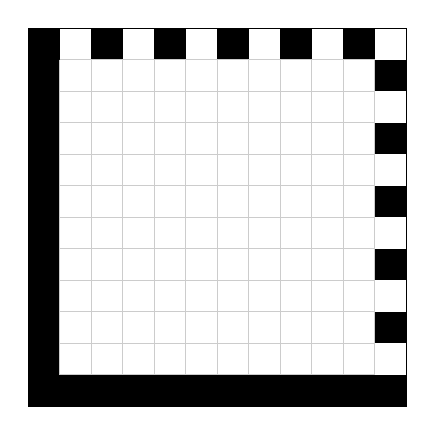
\begin{tikzpicture}[x=4mm, y=-4mm]
  \draw[black] (0,0) rectangle (12,12);
  % L-Pattern: untere Kante + linke Kante
  \foreach \c in {0,...,11}{ \fill[black] (\c, 11) rectangle (\c+1, 12); }
  \foreach \r in {0,...,10}{ \fill[black] (0, \r) rectangle (1, \r+1); }
  % Zeitsignal: obere + rechte Kante alternierend
  \foreach \c in {0, 2, 4, 6, 8, 10}{ \fill[black] (\c, 0) rectangle (\c+1, 1); }
  \foreach \r in {1, 3, 5, 7, 9}{ \fill[black] (11, \r) rectangle (12, \r+1); }
  % Hilfsraster für Datenbereich (transparent grau)
  \foreach \i in {1,...,11}{
    \draw[gray!40, very thin] (\i, 1) -- (\i, 11);
    \draw[gray!40, very thin] (1, \i) -- (11, \i);
  }
\end{tikzpicture}
\end{center}

Die Datenmodule (Innenfläche $10 \times 10$) bleiben leer — das
ist Aufgabe der Etappe 13. Wenn dein Frame an einer Ecke schief
aussieht: das Zeitsignal an der oberen Kante muss \emph{links unten
schwarz} starten (Spalte 0 ist sowieso L-Pattern, also sieht es so
aus, als wäre die obere Kante nur Spalten 2, 4, 6, 8, 10 — was
korrekt ist). Die rechte Kante hat schwarze Module bei Zeilen
1, 3, 5, 7, 9 — Zeile 11 ist L-Pattern.

\subsection*{Bleistift-Übung 3: Smartphone-Scan}

\paragraph{PNG vom Code} Das vom Encoder erzeugte
\texttt{greta.png} (360$\times$360 Pixel mit Quiet-Zone) sollte sich
sowohl auf dem Bildschirm als auch ausgedruckt scannen lassen.
Wenn nicht, prüfe:

\begin{itemize}
\item Ist die Quiet-Zone wirklich um das ganze Symbol herum
  vorhanden? (Bei \texttt{Image.new("L", (360, 360), color=255)}
  und Paste an Position \texttt{(30, 30)} sind es 30 Pixel
  weißer Rand auf jeder Seite.)
\item Wird das PNG im Modus \texttt{"L"} oder \texttt{"RGB"}
  gespeichert? Reine 1-Bit-Bilder lehnen einige Scanner ab.
\item Bildschirm-Helligkeit hoch genug? Bei dunklen Displays
  kann es Kontrast-Probleme geben.
\end{itemize}

\paragraph{Hand-Zeichnung} Die handgezeichnete Variante von Tag 13
ist anspruchsvoller, weil:

\begin{itemize}
\item die Module nicht perfekt quadratisch sind,
\item die Linien des Karopapiers stören (am besten vor dem Scan
  abfotografieren — die Kamera bügelt das meiste glatt),
\item ein einzelnes vergessenes oder zu wenig ausgemaltes Modul
  einen Decoding-Fehler erzeugen kann (Reed-Solomon kann immerhin
  drei Codeword-Fehler reparieren — aber sechs vergessene Module
  in zwei Codewords sind dann doch zu viel).
\end{itemize}

Tipp: ein Foto vom Hand-Symbol mit guter Beleuchtung machen, dann
das Foto am Handy mit der Datamatrix-App scannen. Das funktioniert
oft besser als direkt durch die Kamera auf das Papier zu halten.

\paragraph{Bonus} Wenn beides klappt, hast du gerade einen
kompletten Datamatrix-Workflow durchlaufen — vom Wort über
Berechnung und Zeichnung (oder Druck) bis zum Decode. Damit ist
„Das Geheimnis der Redundanz" für die Praxis-Seite weitgehend
gelöst. Was noch kommt: Aufräumen mit Klassen (Tag 15) und ein
Bonus-Sandkasten mit Decoder und Fehler-Demo (Tag 16).
